  \documentclass[11pt,a4paper,sans]{moderncv}
  \moderncvstyle{banking}
  \moderncvcolor{black}
  \nopagenumbers{}

  \usepackage[utf8]{inputenc}
  \usepackage[top=0.30cm, bottom=0.30cm, left=0.50cm, right=0.50cm]{geometry}
  \usepackage{multicol}
  \usepackage{enumitem}
  \usepackage{amssymb}
  \usepackage{fontawesome5}
  \usepackage{xcolor}
  \usepackage{hyperref}
  \hypersetup{colorlinks=true, urlcolor=black}

  % Custom cventry
  \newcommand*{\customcventry}[7][.10em]{%
  \begin{tabular}{@{}l}
      {\bfseries #4} \\
      {\itshape #3}
  \end{tabular}
  \hfill
  \begin{tabular}{l@{}}
      {\bfseries #5} \\
      {\itshape #2}
  \end{tabular}
  \ifx&#7&%
  \else{\\
  \begin{minipage}{\maincolumnwidth}%
      \raggedright\footnotesize#7%
  \end{minipage}}\fi%
  \par\addvspace{#1}
  }

  \begin{document}
  \raggedright

  % Ultra-compact header: photo left (not in margin), title/info centered and bigger
  \hspace*{0.03\textwidth}% less horizontal space before photo (10% bump back)
  \begin{minipage}[c]{0.13\textwidth}
    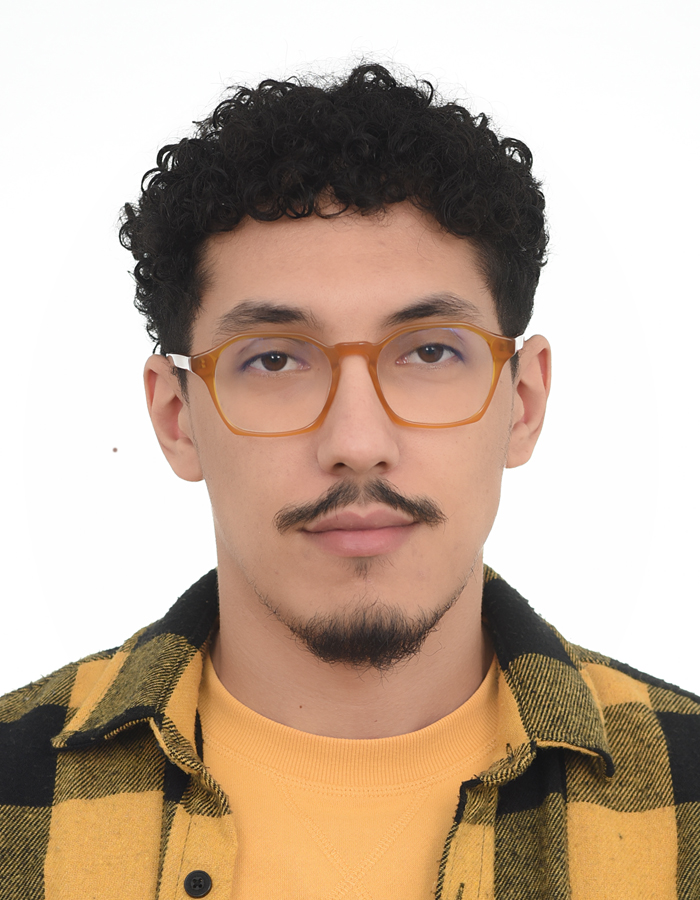
\includegraphics[width=0.85\linewidth]{images/ahmed.jpg}
  \end{minipage}%
  \hfill
  \begin{minipage}[c]{0.84\textwidth}
    \begin{center}
      {\fontsize{20}{22}\selectfont\textbf{Ahmed MAKROUM}}\\[0.7em]
      {\fontsize{13.2}{15.4}\selectfont  Data Engineer – Big Data \& Cloud} \\[0.5em] % <--- Ajouté ici
      {\fontsize{10.5}{12.3}\selectfont
        \faMobile\enspace +212 6 64 71 62 19 \quad
        \faEnvelope\enspace ahmedmakroum3@gmail.com \quad
        \faHome\enspace Casablanca, Maroc \
        \faLinkedin\enspace \href{https://www.linkedin.com/in/ahmed-makroum/}{in/ahmed-makroum} \quad
        \faGithub\enspace \href{https://github.com/ahmedmakroum}{github.com/ahmedmakroum}\quad
        \faGlobe\enspace \href{https://makroum.website}{makroum.website}
      }\\[1em]
    \end{center}
  \end{minipage}
  \vspace{-11pt}

  % PROFIL
  \section{\fontsize{11}\selectfont Profil}
  \vspace{-6pt}
            Ingénieur d’État spécialisé en ingénierie des données, je construis des pipelines fiables et j’automatise les flux pour transformer les données brutes en informations utiles.
            Je développe des systèmes qui aident les équipes à travailler plus efficacement et à prendre de meilleures décisions.
            À la recherche d’un poste pour contribuer à des projets impactants.
            
  % EXPÉRIENCE
  \vspace{-14pt}
  {\renewcommand{\labelitemi}{\raisebox{0.2ex}{\scalebox{1.15}{$\bullet$}}} % +15% size for bullets here only
  \section{\fontsize{11}\selectfont Expérience}
  \vspace{-3pt}

  
  \customcventry{09/2025 ‐ present}{\href{https://metave.ma/}{Metaverse}}{Data Engineer}{}{}{
  \begin{itemize}[leftmargin=0.5cm, itemsep=-2pt, topsep=0pt, partopsep=0pt, parsep=0pt]
  \fontsize{11}{12.3}\selectfont
                \item Conçu des architectures data modulaires sur GCP, AWS et on-premise, standardisant les déploiements clients et réduisant les temps de mise en place.
                \item Automatisé l’infrastructure avec Terraform, supprimant la configuration manuelle et permettant le déploiement d’environnements scalables en quelques minutes.
                \item Mis en place des workflows CI/CD automatisés, garantissant la cohérence et la traçabilité des déploiements entre environnements.
        \end{itemize}}


  \customcventry{03/2025 ‐ 08/2025}{\href{https://www.allianz.ma}{Allianz Maroc}}{Stage - Data Engineer}{}{}{
  \begin{itemize}[leftmargin=0.5cm, itemsep=-2pt, topsep=0pt, partopsep=0pt, parsep=0pt]
  \fontsize{11}{12.3}\selectfont
                \item Conçu et déployé des pipelines NiFi–Spark intégrant plusieurs sources internes dans un entrepôt PostgreSQL unifié, créant une base de données métier centralisée et fiable.
                \item Automatisé les extractions de données pour les équipes métier, supprimant les demandes manuelles et réduisant les délais de livraison des rapports de plusieurs heures à quelques minutes.
                \item Développé une solution de reporting interactive via Metabase, permettant aux utilisateurs de configurer leurs propres tableaux de bord et d’accéder en libre-service à leurs indicateurs clés.
                \item Développé une application microservices (Spring Boot, Next.js) de gestion des règlements santé, avec authentification sécurisée et rôles granulaires, utilisée quotidiennement par 50+ utilisateurs métier.
      \end{itemize}}

  \customcventry{06/2024 ‐ 08/2024}{\href{https://boti.education/}{BOTI School}}{Stage - Data Engineer}{}{}{
  \begin{itemize}[leftmargin=0.5cm, itemsep=-2pt, topsep=0pt, partopsep=0pt, parsep=0pt]
  \fontsize{11}{12.3}\selectfont
                \item Développé un pipeline Apache Beam sur GCP pour traiter et agréger les logs d’utilisation stockés dans des buckets GCS, permettant le suivi précis de la consommation des utilisateurs.
                \item Construit un entrepôt de données sur BigQuery, centralisant les métriques d’usage et automatisant le calcul de la facturation interne par utilisateur.
                \item Créé des dashboards dynamiques dans Looker Studio pour l’équipe financière, offrant une visibilité en temps réel sur les coûts et réduisant le temps de production des rapports de plusieurs heures à quelques minutes.
  \end{itemize}}

  \customcventry{06/2023 ‐ 08/2023}{\href{https://6solutions.com/}{6solutions}}{Stage - Web and Mobile Developer}{}{}{
  \begin{itemize}[leftmargin=0.5cm, itemsep=-2pt, topsep=0pt, partopsep=0pt, parsep=0pt]
  \fontsize{11}{12.3}\selectfont
                \item Développé une plateforme de consulting multi-services (juridique, médical, financier), offrant une solution centralisée pour différents besoins clients 
                \item Réalisé le front-end avec Angular et le back-end avec Spring Boot, assurant une architecture web cohérente
                \item Conçu et déployé la version mobile de l’application en Flutter, permettant un accès fluide aux services depuis n’importe quel appareil
  \end{itemize}}

  \customcventry{07/2022 ‐ 08/2022}{\href{https://estatmar.ma/}{Finso}}{Stage - Game Developer}{}{}{%
  \begin{itemize}[leftmargin=0.5cm, itemsep=-2pt, topsep=0pt, partopsep=0pt, parsep=0pt]
  \fontsize{11}{12.3}\selectfont
                \item Développé un jeu éducatif ludique pour enfants, introduisant des notions de gestion et de stratégie de manière interactive 
                \item Réalisé le projet sous Unity, avec gameplay interactif, animations soignées et interface adaptée, assurant une expérience engageante pour le jeune public
  \end{itemize}}}
  

  % FORMATION
  \vspace{-11pt}
  \section{\fontsize{11}\selectfont Formation}
  \vspace{-4pt}
\noindent
\parbox[t]{0.78\textwidth}{
    \textbf{\href{https://emsi.ma}{EMSI – École Marocaine des Sciences de l’Ingénieur}}, \\
    Diplôme d’Ingénieur d'état en Informatique et Réseaux, option MIAGE 
}
\hfill
\parbox[t]{0.2\textwidth}{
    \raggedleft \textit{09/2020 - 03/2025}
}
\vspace{0.3em}



{}

  % CERTIFICATIONS
  \vspace{-11pt}
  \section{\fontsize{11}\selectfont Certifications}
  \vspace{-5pt}
  \textit{Certifications obtenues via Coursera.}
  \begin{itemize}[leftmargin=0cm, itemsep=-2pt, topsep=0pt, partopsep=0pt, parsep=0pt, label={}]
      \item \textbf{\href{https://www.coursera.org/account/accomplishments/verify/G178XXP17WQA}{Machine Learning with Python}} (IBM)
      \item \textbf{\href{https://www.coursera.org/account/accomplishments/records/M5RKGX36BAVA}{IBM Data Engineering}} (IBM)
      \item \textbf{\href{https://google.com}{Building Scalable Java Microservices with Spring Boot and Spring Cloud}} (Google Cloud)
      \item \textbf{\href{https://www.coursera.org/account/accomplishments/verify/EK5SJM3YM7PX}{Introduction to Big Data with Spark and Hadoop}} (IBM)
      \item \textbf{\href{https://www.coursera.org/account/accomplishments/specialization/B4RCUAYCUG49}{Python for Everybody Specialization}} (University of Michigan)
      \item \textbf{\href{https://www.coursera.org/account/accomplishments/records/G867SJLRFQS2}{Google Business Intelligence}} (Google)
  \end{itemize}

  % COMPÉTENCES
  \vspace{-15pt}
  \section{\fontsize{11}\selectfont Compétences}
  \vspace{-6pt}
  \begin{itemize}[leftmargin=0cm, itemsep=-2pt, topsep=0pt, partopsep=0pt, parsep=0pt, label={}]
    \item \textbf{Data Engineering \& Cloud:} ETL, Big Data (Hadoop, Spark), Airflow, Kafka • GCP, AWS, Docker, Terraform, DataOps
    \item \textbf{Programmation \& Bases de Données:} Python, SQL, Java • PostgreSQL, Hive, MongoDB, Cassandra

  \end{itemize} 

 

  \end{document}

